\chapter{Methodology}
\label{chp:metho}
This paper seeks to determine the best-performing neural network for tool image classification. In the course of the literature review conducted by this paper, no paper about neural networks for tool image classification was found. On that account, the neural network is determined based on the state of the art of neural networks for image classification.
This chapter defines the methodology to determine this neural network. To determine this neural network the state-of-the-art neural networks need to be compared in regard to their performance.
Therefore, a metric, a dataset, and the state-of-the-art neural networks are required.
The metric operationalizes performance. Thus, performance is comparable. The metric is selected and defined in Section \ref{sec:metric}.
The dataset is required to train and evaluate the neural networks. \autocite{LeCun.2015} The methodology of the dataset construction is defined in Section \ref{sec:datasetconstruction}.
This paper focuses on the state of the art of neural networks for image classification, see Section \ref{sec:scope}. The state of the art is analyzed in the course of a literature review conducted by this paper. The methodology of the literature review is defined in Section \ref{sec:litrev}.
The best-performing neural network for tool image classification is determined in the course of an experiment. This experiment is described in Section \ref{sec:experiment}.

\section{Metric}
\label{sec:metric}
Performance of neural networks for image classification is measured on benchmark datasets. The benchmark datasets are listed in Section \ref{sec:benchmark}. For these datasets, performance is measured in classification accuracy or error.\autocites{imagenet.2019}{cifar.2012}{mnist.2010}{svhn.2011}{clothing.2016}{fashionMNIST.2017}{Darlow.2018}{food.2014}{vanHorn.2018}{stanfordcars.2013}{emnistletters.2017}{kuzushijiMNIST.2018}{cub.2011}{Sabour.2017}{isic1.2019}{isic2.2018}{isic3.2018}
Classification accuracy and error are equivalent.\autocite{Bansal.2019b}
Based on these datasets, this paper measures performance in classification accuracy. For reasons of simplification, classification accuracy is referred to as accuracy in the context of this paper. Accuracy is a metric to measure the classification performance of a classifier. Accuracy $acc$ is defined as the amount of correctly predicted labels $correct$ to the total amount of predictions $total$, see Equation \eqref{eq:acc}. \autocite{Bansal.2019b}
\begin{equation}
\label{eq:acc}
acc = \frac{correct}{total}
\end{equation}
\par
As a result, accuracy can be misleading for an imbalanced dataset. For example, given a dataset consisting of $99\%$ samples labeled $A$ and $1\%$ samples labeled $B$, a classifier purely predicting $A$ gets an accuracy of $99\%$. Consequently, this classifier achieves a high accuracy despite predicting all samples labeled $B$ wrong.
The dataset constructed in the course of this paper is balanced. Hence, accuracy is suitable for this dataset.


\section{Dataset Construction}
\label{sec:datasetconstruction}
This paper seeks to determine the best-performing neural network for tool image classification. For this reason, optimally, this paper would construct a huge dataset with various images from different classes of tools.\autocites{Howard.2013}{cifar.2012}{imagenet.2019}  
However, time and resources of this paper are limited. Labeling huge amounts of data, such as data mined from the web, requires resources. On that account, this paper exclusively uses labeled data to construct the dataset. Labeled data can be acquired from already existing datasets and from creating inherently labeled images.
\par
This paper creates inherently labeled images. Inherently labeled images are created by taking all images of one class before taking images of another class and storing them in different folders. The resulting folder structure is comprised by a root folder containing one folder for each image class. The classes were chosen based on the available tools. The resulting classes are listed below.
\begin{itemize}
	\item drill
	\item hammer
	\item pliers
	\item saw
	\item screwdriver
	\item wrench
\end{itemize}
The dataset is constructed for a tool image classification task. Thus, the created images each consist of exactly one tool. In real world scenarios, tools are presented from various angles and with various backgrounds. Due to this, the created images are taken from arbitrarily chosen angles and with arbitrarily chosen backgrounds. 
\par
A local joinery provided tools and the location for the creation of the dataset free of charge. The dataset was created by placing a tool in an arbitrarily chosen position and taking a series of close-up images. During the series, the camera was moved around the tool to create arbitrary angles. For the next series, the tool, the background, and/or the position of the tool was changed. 
The images were created by volunteers and the author of this paper: Nina Eichler, Sophia Fai{\ss}t, Manuel Krumbacher, and Fabian Wolf. 
The resulting dataset is provided publicly available under the Creative Commons Attribution-ShareAlike 4.0 International License. The dataset is appended in the digital appendix, see Section \ref{sec:digiappend}. The dataset is described in Section \ref{sec:experiment}

\section{Literature Review}
\label{sec:litrev}
The literature review consists of a preparation and an implementation phase.
In the preparation phase, literature inclusion and exclusion criteria, a literature source list, and a term table are constructed.
The inclusion and exclusion criteria determine whether or not a paper is selected for the literature review. The inclusion and exclusion criteria are listed in Section \ref{sec:krit}.
The literature source list lists all sources of papers. These sources are journals, conference proceedings, full-text databases, image classification leaderboards, and scientific search engines. The literature source list is displayed in Section \ref{sec:source}.
The term table lists terms related to the problem statement described in Section \ref{sec:problem}. As a result, the term table contains all terms that can be used to derive search queries. The term table is displayed in Section \ref{sec:termtable}.
In the implementation phase, the sources are systematically screened using the search queries. The resulting papers are selected using the inclusion and exclusion criteria. Following \cite{Webster.2002}, the selected papers are analyzed in Concept Matrix \ref{tab:concept_matrix}. The concept matrix maps each paper to concepts of neural networks they support.
\par
The state-of-the-art neural networks for image classification are selected based on these concepts. For each concept this paper determines the best-performing neural network for image classification. Performance of neural networks for image classification is measured on benchmark datasets. The benchmark datasets are listed in Section \ref{sec:benchmark}. For these datasets, neural networks are ranked on leaderboards based on accuracy. The accuracy differs for the same neural network on different leaderboards. Accordingly, different leaderboards have differently complex tasks. Thus, neural networks cannot be compared by averaging accuracy across all leaderboards. Furthermore, not every neural network is listed on every leaderboard. \autocites{imagenet.2019}{cifar.2012}{mnist.2010}{svhn.2011}{clothing.2016}{fashionMNIST.2017}{Darlow.2018}{food.2014}{vanHorn.2018}{stanfordcars.2013}{emnistletters.2017}{kuzushijiMNIST.2018}{cub.2011}{Sabour.2017}{isic1.2019}{isic2.2018}{isic3.2018} Hence, the neural networks are not comparable by averaging rank across all leaderboards. Accordingly, the neural networks are compared pairwise. A neural network $A$ is ranked above a neural network $B$ if $A$ performs better on a larger number of leaderboards that contain both $A$ and $B$.
\par
Neural networks ranked on the leaderboards use different auxiliaries to further improve performance. \autocites{Lim.2019}{Harris.2020}{Huang.2019b}{Wang.2019}{Xie.2019b}{Touvron.2019}{Darlow.2018}{Tan.2019}
As stated in Section \ref{sec:scope}, this paper focuses exclusively on the neural network. Therefore, only the underlying neural network is regarded. If several versions of the underlying neural network exist, the best-performing version according to the paper originally proposing the neural network is regarded as the best-performing state-of-the-art neural network.
\par
In summary, the result of this literature review are state-of-the-art concepts of neural networks for image classification and the best-performing state-of-the-art neural network for each concept. The results of the literature review are reported in Chapter~\ref{chp:sota}.


\section{Experiment}
\label{sec:experiment}
This paper seeks to determine the best-performing neural network for tool image classification. The best-performing neural network is determined in the course of an experiment. The experiment is conducted by training and evaluating selected neural networks on a dataset. The Dataset, selected neural networks, training, and evaluation are described in this chapter. To measure performance, accuracy is used, see Section \ref{sec:metric}. The results of this experiment are reported in Chapter~\ref{chp:result}. To conduct the experiment, Movilizer GmbH provided $200$ hours on an Amazon Web Service g4dn.xlarge instance running a Deep Learning AMI (Ubuntu 18.04).\autocite{AWS.2020a}
The g4dn.xlarge instance provides 4 vCPUs, 16GB RAM, 125GB storage, and a NVIDIA~T4~GPU. \autocite{AWS.2020b} 
The experiment is implemented in Python 3\autocite{Python3} using Keras~2.2.4.2\autocite{Keras}, Tensorflow 2.1.0\autocite{Tensorflow.2015}, CUDA 10.1\autocite{CUDA}, and cuDNN\autocite{cuDNN}. The dataset and code used to conduct the experiment are appended in the digital appendix, see Section \ref{sec:digiappend}.

\subsection{Dataset}
The dataset is constructed as described in Section \ref{sec:datasetconstruction}. The constructed dataset is comprised of tool images for image classification. Therefore, it is named \ac{TIC Dataset}. The \ac{TIC Dataset} is comprised of $20{,}400$ tool images of six classes. The classes are listed below.
\begin{itemize}
	\item drill
	\item hammer
	\item pliers
	\item saw
	\item screwdriver
	\item wrench
\end{itemize}
Each class comprises $3{,}400$ tool images. A tool image is a close-up image of exactly one tool. 
For a class, tool images display different tools of the same class from arbitrary angles and with arbitrary backgrounds. Figure \ref{fig:screwdriver} illustrates this for the class screwdriver with two images of different tools.
\begin{figure}[H]
	\centering
	\begin{subfigure}[b]{0.45\textwidth}
		\centering
		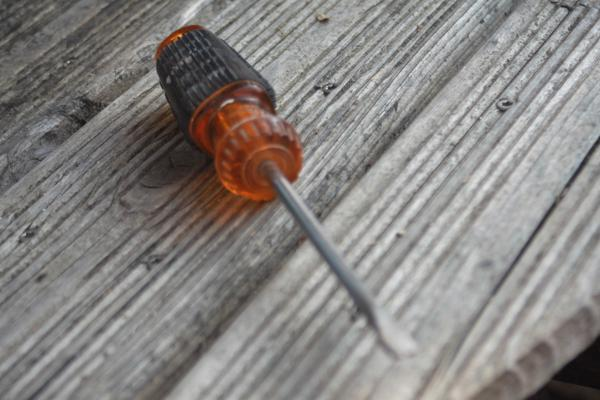
\includegraphics[width=\textwidth]{img/screwdriver1}
	\end{subfigure}
	\hfill
	\begin{subfigure}[b]{0.45\textwidth}
		\centering
		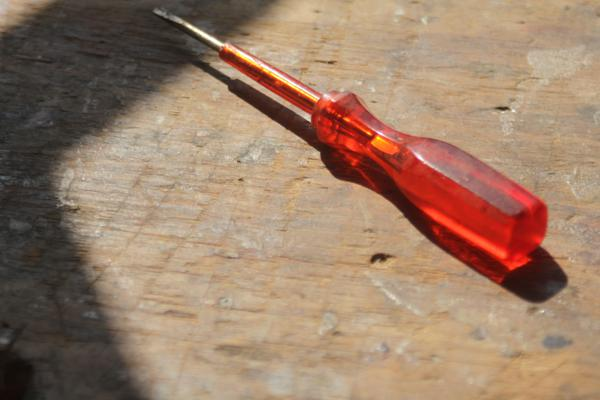
\includegraphics[width=\textwidth]{img/screwdriver2}
	\end{subfigure}
	\caption{Two Images from the TIC Dataset of Class Screwdriver (own figure)}
	\label{fig:screwdriver}
\end{figure}
The dataset is split into a training, validation, and test dataset. For each class, $60\%$ of the images are randomly split for the training dataset, $20\%$ for the validation dataset, and $20\%$ for the test dataset. The resulting training dataset contains $12{,}240$, the resulting validation dataset contains $4{,}080$, and the resulting test dataset contains $4{,}080$ images. For each of these datasets, the images are evenly distributed over all classes.
The training dataset is used to train a neural network. The validation dataset and the test dataset are not used for training. On that account, the neural network cannot overfit to the validation dataset and the test dataset. Thus, the validation dataset can be used to explore different hyperparameters and monitor whether or not the neural network overfits to the training dataset. Based on the performance on the validation dataset, the neural network is chosen for evaluation. This way, the neural network might develop a dependency on the validation dataset. For example, a neural network might perform well on the validation dataset by chance but less well on other data. For this reason, the neural network is evaluated only once on the test dataset. The performance of  the neural network on the test dataset is regarded as the performance of the neural network. \autocite{ElAmir.2020}



\subsection{Neural Network Selection}
To determine the best-performing neural network for tool image classification, optimally, this paper would conduct a neural network architecture search and hyperparameter search. However, resources and time of this paper are limited. Due to that, conducting a neural network architecture search and hyperparameter search is not possible. 
\par
Tool image classification is a sub-task of image classification. Therefore, this paper selects the state-of-the-art neural networks for image classification to conduct the experiment. The state-of-the-art neural networks for image classification are determined as described in Section \ref{sec:litrev}. For each selected neural network the network architecture and the hyperparameters are adopted from the paper originally proposing the neural network. The following neural networks are selected to conduct the experiment:
\begin{itemize}
	\item VGG-19, see Section \ref{sec:conv}. \autocite{Simonyan.2014}
	\item ResNet-152, see Section \ref{sec:res}. \autocite{He.2016}
	\item ResNext-101, see Section \ref{sec:inception}. \autocite{Xie.2017}
	\item DenseNet-264, see Section \ref{sec:dense}. \autocite{Huang.2017}
	\item EfficientNet-B7, see Section \ref{sec:sepconv}. \autocite{Tan.2019}
\end{itemize}
This paper implements the selected neural networks based on their Keras implementation.\autocite{KerasApp} Note that CapsNet is excluded since it does not reach state-of-the-art performance on image classification except for classification of digits or letters.



\subsection{Training}% Training Hyperparams
The neural networks are trained on the training dataset and their performance is monitored on the validation dataset.
Training is carried out by optimizing the categorical cross entropy loss function \autocites{Michelucci.2019}{ElAmir.2020}{Singh.2020}, see Section \ref{sec:training}. Each selected neural network is trained with the number of epochs, the optimizer, and the hyperparameters of the optimizer as specified in the paper originally proposing the neural network.
The hyperparameters of the optimizer are initial learning rate, learning rate schedule, and momentum or Nesterove momentum if used. The learning rate schedule determines how the learning rate changes with epochs progressing.
The batch size specified in the original papers are powers of 2. However, those batch sizes are too large to fit the available GPU. Therefore, the power is reduced by one until the batch size fits the available GPU. For each neural network, the training hyperparameters, namely number of epochs, the optimizer, the hyperparameters of the optimizer, and the batch size are displayed in Table \ref{tab:hyperparams}. \autocites{Simonyan.2014}{He.2016}{Xie.2017}{Huang.2017}{Tan.2019}
\par
For EfficientNet-B7, the number of epochs is not specified, instead EfficientNet-B7 is trained until convergence. \autocite{Tan.2019} The available $200$ hours on the provided hardware might not be enough to train EfficientNet-B7 until convergence. Therefore, the other neural networks are trained before EfficientNet-B7. EfficientNet-B7 is trained for the remaining time.
\begin{xltabular}{\textwidth}{llX}\toprule
	\caption[Training Hyperparameters]{Training Hyperparameters \autocites{Simonyan.2014}{He.2016}{Xie.2017}{Huang.2017}{Tan.2019}} \label{tab:hyperparams}\\
	\textbf{Neural Network} & \textbf{Training Hyperparameters} & \\\midrule \endhead
	VGG-19 & Epochs: & $74$\\
		& Optimizer: & \ac{SGD}\\
		& Initial Learning Rate: & $0.01$\\
		& Learning Rate Schedule: & divide learning rate by $10$ on accuracy plateaus.\\
		& Momentum: & $0.9$\\
		& Batch Size: & $32$\\
	\\\midrule
	ResNet-152 & Epochs: & $120$\\
		& Optimizer: & \ac{SGD}\\
		& Initial Learning Rate: & $0.1$\\
		& Learning Rate Schedule: & divide learning rate by $10$ on accuracy plateaus.\\
		& Momentum: & $0.9$\\ 
		& Batch Size: & $32$\\
	\\\midrule
	ResNeXt-101 & Epochs: & $120$\\
		& Optimizer: & \ac{SGD}\\
		& Initial Learning Rate: & $0.1$\\
		& Learning Rate Schedule: & divide learning rate by $10$ at epoch $30$, $60$, and $90$.\\
		& Momentum: & $0.9$\\ 
		& Batch Size: & $16$\\
	\\\midrule
	DenseNet-264 & Epochs: & $90$\\
		& Optimizer: & \ac{SGD}\\
		& Initial Learning Rate: & $0.1$\\
		& Learning Rate Schedule: & divide learning rate by $10$ at epoch $30$ and $60$.\\
		& Nesterov Momentum: & $0.9$\\
		& Batch Size: & $32$\\
	\\\midrule
	EfficientNet-B7 & Epochs: & not specified\\
		& Optimizer: & \ac{RMSProp}\\
		& Initial Learning Rate: & $0.256$\\
		& Learning Rate Schedule: & decay learning rate by $0.97$ each $2.4$ epochs.\\
		& Momentum: & $0.9$\\
		& Batch Size: & $1$
	\\\bottomrule
\end{xltabular}
Note that metalearning, semi- or unsupervised learning, transfer learning, adversarial training, data augmentation, input normalization, weight decay, and multi-task learning are excluded from the scope of this paper,  see Section \ref{sec:scope}. In consequence, they are excluded from the experiment even if they are used in the original papers.

\subsection{Evaluation}
As mentioned, during training the performance of each neural network is monitored on the validation dataset. The performance is measured at the end of each epoch. After training for the entire number of epochs, the neural network from the epoch with the highest performance is evaluated. A neural network is evaluated on the test dataset. The resulting performance measured in accuracy is reported in Chapter \ref{chp:result}.
